% !TEX root = ../numapde-OptiPuls.tex

\newcommand{\varR}{2.5}
\newcommand{\varr}{1}
\newcommand{\vardi}{0.5}
\newcommand{\vardii}{0.8}
\newcommand{\varrlas}{0.4}
\newcommand{\varhlas}{0.8}

\definecolor{mycoral}{RGB}{236,27,75}
\definecolor{myorange}{RGB}{242,106,68}

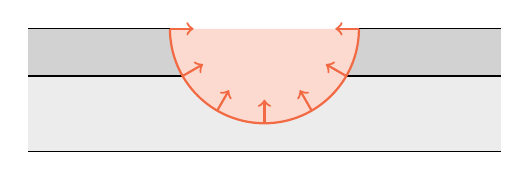
\begin{tikzpicture}[scale=1.2]

	% fillers
	\draw [draw=none, fill=gray!35] (-\varR,0) rectangle (\varR,-\vardi);
	\draw [draw=none, fill=gray!15] (-\varR,-\vardi) rectangle (\varR,-\vardi-\vardii);

	% lines
	\draw (-\varR,-\vardi) -- (\varR,-\vardi);
	\draw (-\varR,-\vardi-\vardii) -- (\varR,-\vardi-\vardii);
	\draw (-\varR,0) -- (-\varr,0);
	\draw (\varr,0) -- (\varR,0);

	\draw [myorange, thick, fill=myorange!25] (0,0) ++(180:\varr) arc (180:360:\varr);

	% velocity
	% \foreach \angle in {-180, -135, -90, -45, 0}
	\foreach \angle in {-180, -150, -120, -90, -60, -30, 0}
	{
		\draw [->, myorange, thick] ({\varr*cos(\angle)}, {\varr*sin(\angle)}) -- ({0.75*\varr*cos(\angle)}, {0.75*\varr*sin(\angle)});
	}

\end{tikzpicture}
